\section{Graphs}

Graphs have \verb|n| vertices $V$ and \verb|m| edges $E$.

\begin{enumerate}
    \setlength{\itemsep}{0em}
    \item \textbf{Adjacent(u,v)}: Return wheter there is an edge from vertices \verb|u| to \verb|v|.
    \item \textbf{Neighbors(u)}: Return list of all vertices \verb|v| with edges from \verb|u|.
    \item \textbf{Insert(v,u)}: Insert an edge from vertex \verb|v| to vertex \verb|u|.
\end{enumerate}

\subsection{Representations}
\label{sec:graph-representations}
\subsubsection{Adjacency matrix}
\verb|n| $\times$ \verb|n| boolean matrix where \verb|mat[u][v]| is true if there is an edge from vertex \verb|u| to vertex \verb|v|. Efficient for dense graphs.

\timeComplexity{1,n,1}
\spaceComplexity{n^2}

\subsubsection{Adjacency list}
Array of size \verb|n| containing linked lists of neighbors. \\
Efficient for sparse graphs.\footnote{Almost all real-world graphs are sparse}

\timeComplexity{\deg(v)}
\spaceComplexity{n + m}

\subsection{Search}
\subsubsection{Depth-first search (DFS)}
\begin{enumerate}
    \setlength{\itemsep}{0em}
    \item Pick a node.
    \item Add all unseen neighbors to stack.
    \item Pop from stack and repeat until stack is empty.
\end{enumerate}

Nodes can be unmarked, seen, or visited. Unmarked nodes are not in stack, seen nodes are in stack, and visited nodes have been popped from stack.

\begin{python}
def dfs(graph, start): # Adjacency list and starting vertex.
    visited = set()
    stack = [start]

    while stack:
        vertex = stack.pop()
        if vertex not in visited: # Since we uncritically add neighbors to the stack.
            visited.add(vertex)
            stack.extend(graph[vertex] - visited) # Add all unvisited neighbors to stack.

    return visited
\end{python}

\timeComplexity{n + m}
\spaceComplexity{n}

\subsubsection{Breadth-first search (BFS)}
Like DFS but uses a queue instead of a stack. Finds the shortest path in an unweighted graph.

\begin{python}
def bfs(graph, start):
    visited = set()
    queue = [start]

    while queue:
        vertex = queue.pop(0)
        if vertex not in visited:
            visited.add(vertex)
            queue.extend(graph[vertex] - visited) # Add unvisited neighbors to the queue.

    return visited
\end{python}

\timeComplexity{n + m}
\spaceComplexity{n}

\subsection{Applications}
Assuming we use adjacency lists.
\subsubsection{Count connected components}
Run DFS or BFS on any unvisited vertex and count how many times you have to run it to visit all nodes.

\timeComplexity{n + m}

\subsubsection{Shortest path}
In an unweighted graph, a BFS tree finds a shortest path\footnote{There can be multiple shortest paths, BFS will find one of them}
from the starting vertex to all other vertices.

\timeComplexity{n + m}

\subsubsection{Distance}
By giving each vertex a distance field, we can find the distance from the starting vertex to all other vertices.

\begin{python}
def bfs_with_distance(graph, start):
    visited = set()
    queue = [start]
    start.dist = 0 # Set distance of starting vertex to 0.

    while queue:
        vertex = queue.pop(0)
        if vertex not in visited:
            visited.add(vertex)
            for neighbor in graph[vertex]:
                if neighbor not in visited:
                    queue.append(neighbor)
                    neigbor.dist = vertex.dist + 1

\end{python}

\timeComplexity{n + m}

\subsubsection{Bipartiteness}
A graph is bipartite if it can be colored with two colors such that no adjacent vertices are the same color.
$\implies$ the graph has no even-length cycles.

\begin{python}
def is_bipartite(graph):
    bfs_with_distance(graph, start) 
    # Run BFS to find distance of all vertices from starting vertex.
    for vertex in graph:
        for neighbor in graph[vertex]:
            if vertex.dist % 2 == neighbor.dist % 2: 
                # If two adjacent vertices are both odd/even distance from the starting vertex, then they are the same color and the graph is not bipartite.
                return False
\end{python}

\timeComplexity{n+m}

\section{Directed Graphs}

\subsection{Representations}
Like with undirected graphs in \ref{sec:graph-representations}, we can use matrices and linked lists. 

\subsection{Topological sort}
A topological sort is a sort such that all vertices only point to vertices that come after them in the sort. \\

To execute a topological sort:
\begin{enumerate}
    \setlength{\itemsep}{0em}
    \item Find vertex with in-degree 0. Remove it from the graph and add it to the sort.
    \item Repeat until all vertices are removed.
\end{enumerate}

\subsubsection{Implementations}

\textbf{1. Reverse Graph}
Take the adjacency list and construct a reverse graph. Then go through the array to find vertices with in-degree 0 and add them to the sort. Remove them from the graph and repeat until all vertices are removed.

\timeComplexity{n^2}

\textbf{2. In-degree array}
Maintain the in-degree of each vertex in an array. Initially, add all vertices with in-degree 0 to a queue. Then repeatedly pop from the queue, add the vertex to the sort, and decrease the in-degree of its neighbors. If any neighbor's in-degree becomes 0, add it to the queue.

\timeComplexity{n + m}

\subsubsection{DAGs}
A topological sort is possible $\iff$ the graph is a DAG.\footnote{directed acyclic graph}

\subsection{Automata}
Automata are directed graphs where edges have values, and a path from a starting vertex to an ending vertex represents a string of values.

$a,b,c, \cdots$ are values, and $\epsilon$ means no value.

Regular expressions can represent all possible paths on the automata.

\textbf{Components of regular expressions}:
\begin{list}{}{}
    \setlength{\itemsep}{0em}
    \item $a \cdot b$ : $a$ followed by $b$.
    \item $a | b$ : $a$ or $b$.
    \item $a^*$ : $a$ repeated 0 or more times.
    \item $a^+$ : $a$ repeated 1 or more times.
\end{list}

\begin{figure}[h]
    \centering
    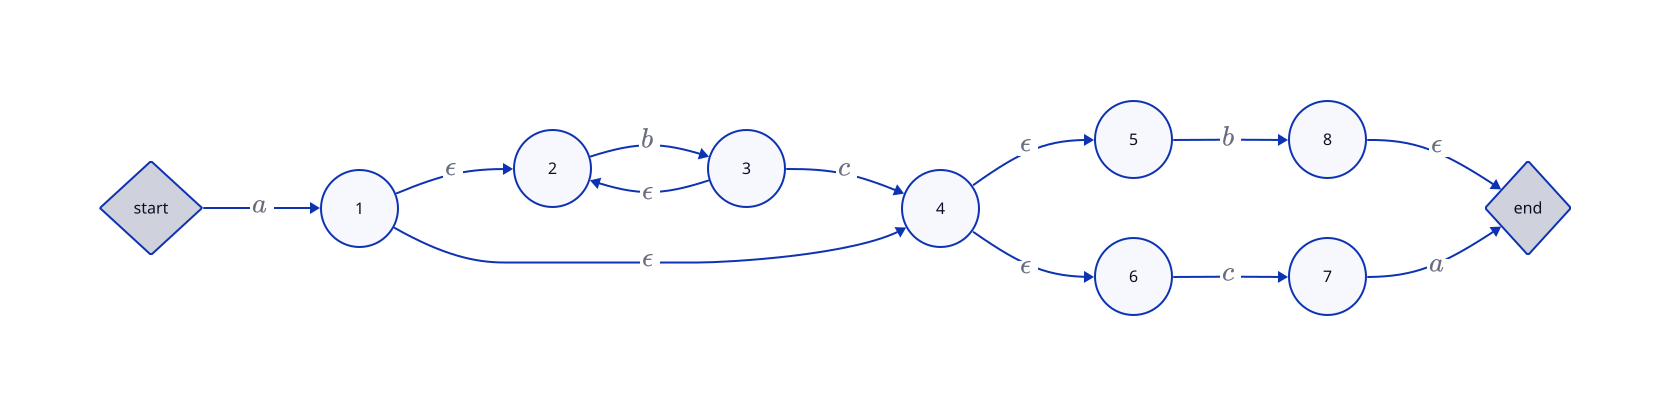
\includegraphics[width=\linewidth]{Assets/res/automata}
    \caption{Automata with the regular expression 
    $a \cdot ((b^* \cdot c) | \epsilon) \cdot (b | (c \cdot a))$}
\end{figure}

\subsection{Strongly connected components}
A strongly connected component is a maximal subgraph where there is a path from any vertex to any other vertex.